\section{Validation Metrics}
We found our pipeline to be an effective tool to beautify images of urban spaces. We now want to understand what the algorithm is looking at when transforming images. Given the limited 
 
%One of the main contribution of this work is developing metrics, which can to a high degree of certainty, explain what the network is learning to be discriminatory features of beauty. We summarize some metrics mentioned in the table \ref{tab:Design_metrics}, which are taken from 
%urban design literature. 
%To test the different hypotheses, we use the balanced sample of 1000 images which rank on the extreme fringes of the Trueskill scores distribution and then transform these images towards the opposite side of the distribution . So an ugly image, according to its Trueskill score, would be transformed into a beautiful images and vice versa. Once the transformation is done, we measure different computational metrics and compare
%them between these two transformed groups. The differences in these metrics give us a good understanding of what the deep learning model is learning about the concept if beauty in an urban setting. 
The table \ref{tab:Design_metrics} shows a list of design metrics, which are taken from urban design literature. Apart from being interpretable, these metrics also have an important property which is measurability. All of these metrics have an approximate way of measurement using one or more of the computer the state of art computer vision tools. In this section we try to elaborate on the computational methods used to measure the metrics and the results that we get on the pre and post transform images. 

\begin{table*}[h]
	\centering
	
	\resizebox{\linewidth}{!}{%
		\begin{tabular}{|c|p{14cm}|}
			\hline
			\textbf{Metric} & \textbf{Description}\\
			\hline
			
			Walkability  & Walkable streets are rated high on an affective scale. Walkable streets increase the social capital of a place and appeals to the exploring nature of human psyche. This implies that the urban space needs to engage a fundamental need of people to walk and explore. This also implies that a walkable street must also be perceived as safe.\\
			\hline
			Visual Complexity & Visual complexity is a measure of how diverse a urban scene is. It manifests in terms of various design materials, textures and objects. Generally Visual complexity has an inverse 
			'U' relation with affective values. The beauty and aesthetics of a place increases until it starts dropping because of 'too much' complexity \\
			\hline
			Privacy-Openness &  A sense of privacy and a complimentary sense of open-ness are both influential in our perception of a place. These values also tend to be related in an inverse 'U' fashion with beauty\\ 
			\hline
			Green Spaces & Presence of Greenery is always pleasing to the eye. The literature always links curated and well maintained green spaces, where social interactions can happen, to be elements that bring a place 
			together. This implies that dense forests or unkempt greens are not always related to the sense of beauty in urban scenes. \\
			\hline
			Landmarks & Loosing a bearing in the city is not a very pleasant experience. Hence presence of recognizable and easy to look at landmarks influences the perception of an urban space\\
			
			\hline
	\end{tabular}}
	\caption{Urban Design Metrics}
	\label{tab:Design_metrics}
	%        \vspace{-5mm}
\end{table*}


\subsection{Computational Methods}

To validate the metrics mentioned in Table \ref{tab:Design_metrics} computationally we use out of the box deep learning tools like PlacesNet \cite{zhou2014learning} and Segnet \cite{badrinarayanan2015segnet}. 
These two frameworks allow us to extract the type of scene in the image as well as different elements in the image like road, buildings , trees etc and scene types like Plaza, 
\subsubsection{Prevalence Plots}
We use the data that is transformed into beautiful and ugly scenes using the learned model, to analyze scene level characteristics. To understand the scene level properties, we use PlacesNet \cite{zhou2014learning} , to infer the top 5 labels from a set of 205 scene labels. We further classify the 205 labels into 4 salient categories abbreviated \textbf{L}andmarks , \textbf{A}rchitectural , \textbf{W}alkable , \textbf{N}atural. Each category is inspired from the urban design measurement book \cite{urbanDesign}.  Labels like \textit{Abbey , Plaza , Courtyard, Garden, Picnic Area, Park , etc} fall into the category of \textit{Walkable}, where as labels like \textit{Mansion, Castle, Dam , Airport, etc} fall in the category of \textit{Landmarks}. Labels like \textit{Residential neighborhood, Motel, hotel, restaurant, etc} fall in the category of \textit{Architectural} and labels like {fields, pasture , forest, ocean, beach etc } fall in the category \textit{natural}. All in all the labels represent the most broad urban design motifs that constitute a livable city. 
The next step was to compare prevalence , or over expression of these labels and categories in beautified images compared to uglified images. Because the transformation is directly dependent on maximizing the classifier's certainty about an image being beautiful or ugly, this method directly gives us an proxy about what according to the classifier constitutes and beautiful or ugly urban scene.


\subsubsection{Logistic Regressions}

To understand the predictability and interdependence between the most influencing objects in an image and the probability of finding an image beautiful, we adapt the approach as described in \cite{vaughn2008data},
which proposes using logistic regression coefficients as a measure for upper bounds on influence of a variable. This method is also helpful in understanding the interdependence of variables for a particular outcome. 
Using the approach we perform a logistic regression over the two variables $V_1$ and $V_2$ which denote the ratio of a particular type of object pixels to the total area of image in pixels. So these ratios basically represent how much of the total image area is dominated by a particular object. The objects in this study are limited to the 12 urban object labels supported by SegNet \cite{badrinarayanan2015segnet}.
Assuming dependence, we introduce  a third term, which represents the factor that measures the dependence of $V_1$ and $V_2$ and is simply the product $V_1 * V_2 $.
The logistic regression would try to fit a line 
\begin{equation}
L = invLogit(\alpha + \beta_1 * V_1 + \beta_2 * V_2  + \beta_3 * V_{1}.V_{2} )
\label{eq:regression} 
\end{equation}
Here $invLogit$ is the inverse Logistic function. According to the rule of fourth described in \cite{vaughn2008data} , the coefficients $ \beta_1, \beta_2 and \beta_3 $ represent some properties about the influence of $ V_1, V_2 $. An increase in 1\% area of the amount of pixels belonging to object $ V_2 $ would correspond to a maximum increase/decrease of $\frac{\beta_2}{4}$ percent in the likely hood of the image being beautiful. Same rule applies for $\beta_1$. In case of $\beta_3$ the co-efficient corresponds to mutual dependence. An intuitive explanation is that if a 1\% change in value of $V_1$ would add $\beta_3$ to the value of $\beta_2$. Hence $\beta_3$ links changes in variable $V_1$ to changes in influence of variable $V_2$ and vice versa.
We perform the logistic regression on the 5 prime influences namely \textit{Sky , Buildings , Road , Vehicles , Trees}. The results of pairwise regression along with the dependency term are summaries in the table \ref{tab:regressioncoef}
\begin{table}[h]
	\centering
	\begin{tabular}{|c|c|c|c|c|}
		\hline
		\textbf{Object pair} & \textbf{$\beta_1$}  & \textbf{$\beta_2$} & \textbf{$\beta_3$}  & Error Rate (Percentage)\\
		\hline
		\hline
		Roads - Vehicles  & -0.015  & -0.05 & 0.023  & 40.6 \\
		\hline
		Sky - Buildings & -0.08 & -0.11 & 0.064 & 14.4 \\
		\hline
		Sky - Trees & 0.03 & 0.11 & -0.012 & 12.8  \\
		\hline
		Buildings - Trees & -0.032 & 0.084  & 0.005  & 12.7 \\
		\hline
		Roads - Trees & 0.04  & 0.10 &  -0.031  & 13.5  \\
		\hline
		Roads - Buildings & -0.05  & -0.097  &  0.04  & 20.2  \\
		\hline
	\end{tabular}
	\caption{Regression coefficients}
	\label{tab:regressioncoef}
	%        \vspace{-5mm}
\end{table}



\subsubsection{Binned Plots}
\label{sec:Binned}
To understand the relationship between a metric and beauty in urban scenes, we employ the technique of binned plots. We do this by first transforming 500 images from both sides of the beauty spectrum to either beautiful or ugly images. We then find the range across which a particular metric varies across the 1000 images. This range is broken into bins and then each image out of the 1000, is assigned to a particular bin, based on where the value of its metric falls. We then repeatedly sample 100 images across each bins, and count how many of the sampled images fall in either beauty or ugly transformed category. We plot the mean and standard error in a plot for these occurrence frequencies. The resulting plot gives a trend about how likely is a metric favoured or disfavoured by the beautification process.


\subsection{Walkability and Green spaces}
As mentioned in table \ref{tab:Design_metrics} , Walk-ability of streets has high impact on the beauty and other aesthetic qualities of a place. We try to test this by hypothesizing about the impact of green spaces and walkability on beauty.
\par
\textit{[H1] Walkable streets is favoured in beautiful urban scenes}
\par
To test that \textit{H1} is valid, we first plot a prevalence count of different categories of labels for Beautified and uglified images. These labels are scene types extracted using the PlacesNet deep convolutional network \cite{zhou2014learning}. The labels are then classified into taxonomical classes of Landmarks, Architectural, Walkable and Natural classes.  It can be seen from Fig \ref{fig:taxonomyCount}, that walk able scene types are highly favoured in the beautification process. Ugly images are transformed into Walkable spaces almost twice as frequently in beautification compared uglification.
\begin{figure}[h]
	\centering
	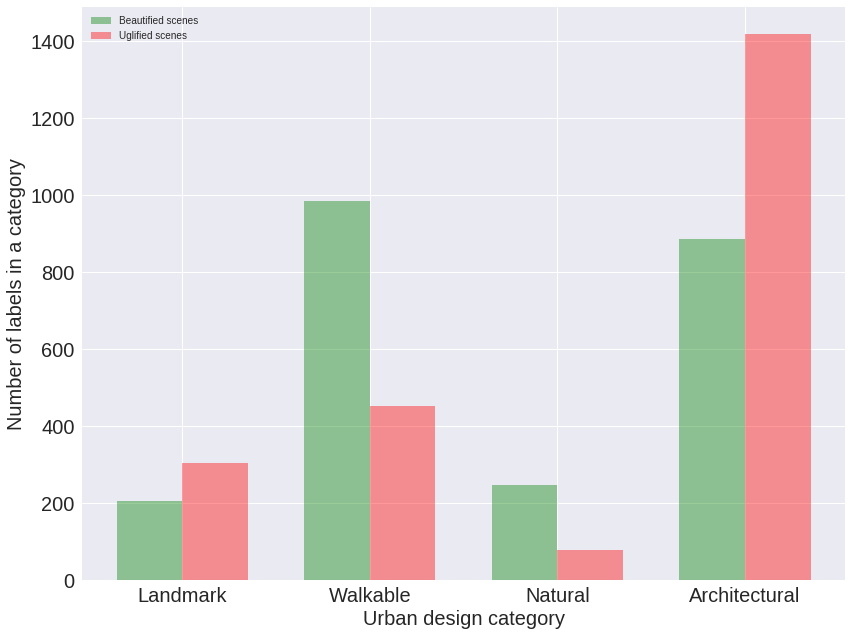
\includegraphics[width=\columnwidth]{Plot/taxonomyCount.png}
	\caption{Prevalence plot of categories of scenes prevalent in Beautified against Ugly-fied images}
	\label{fig:taxonomyCount}
\end{figure}

\par
\textit{[H2] Green spaces are favourable for beauty in urban scenes.  }
\par

Figure \ref{fig:taxonomyCount} and \ref{fig:WalkableTnomy} implies that natural scene are twice as likely in beautified images than in uglified images. But to test this hypothesis further, we plot a binned plot for greenery pixels in images across the transformed image datasets. It can be seen from Fig \ref{fig:greenBinned} that as the green cover in an urban image increases, it is highly favoured in beautified class than in the uglyfied class. This shows that the green spaces are highly favourable for urban beauty.

\begin{figure}[h]
	\centering
	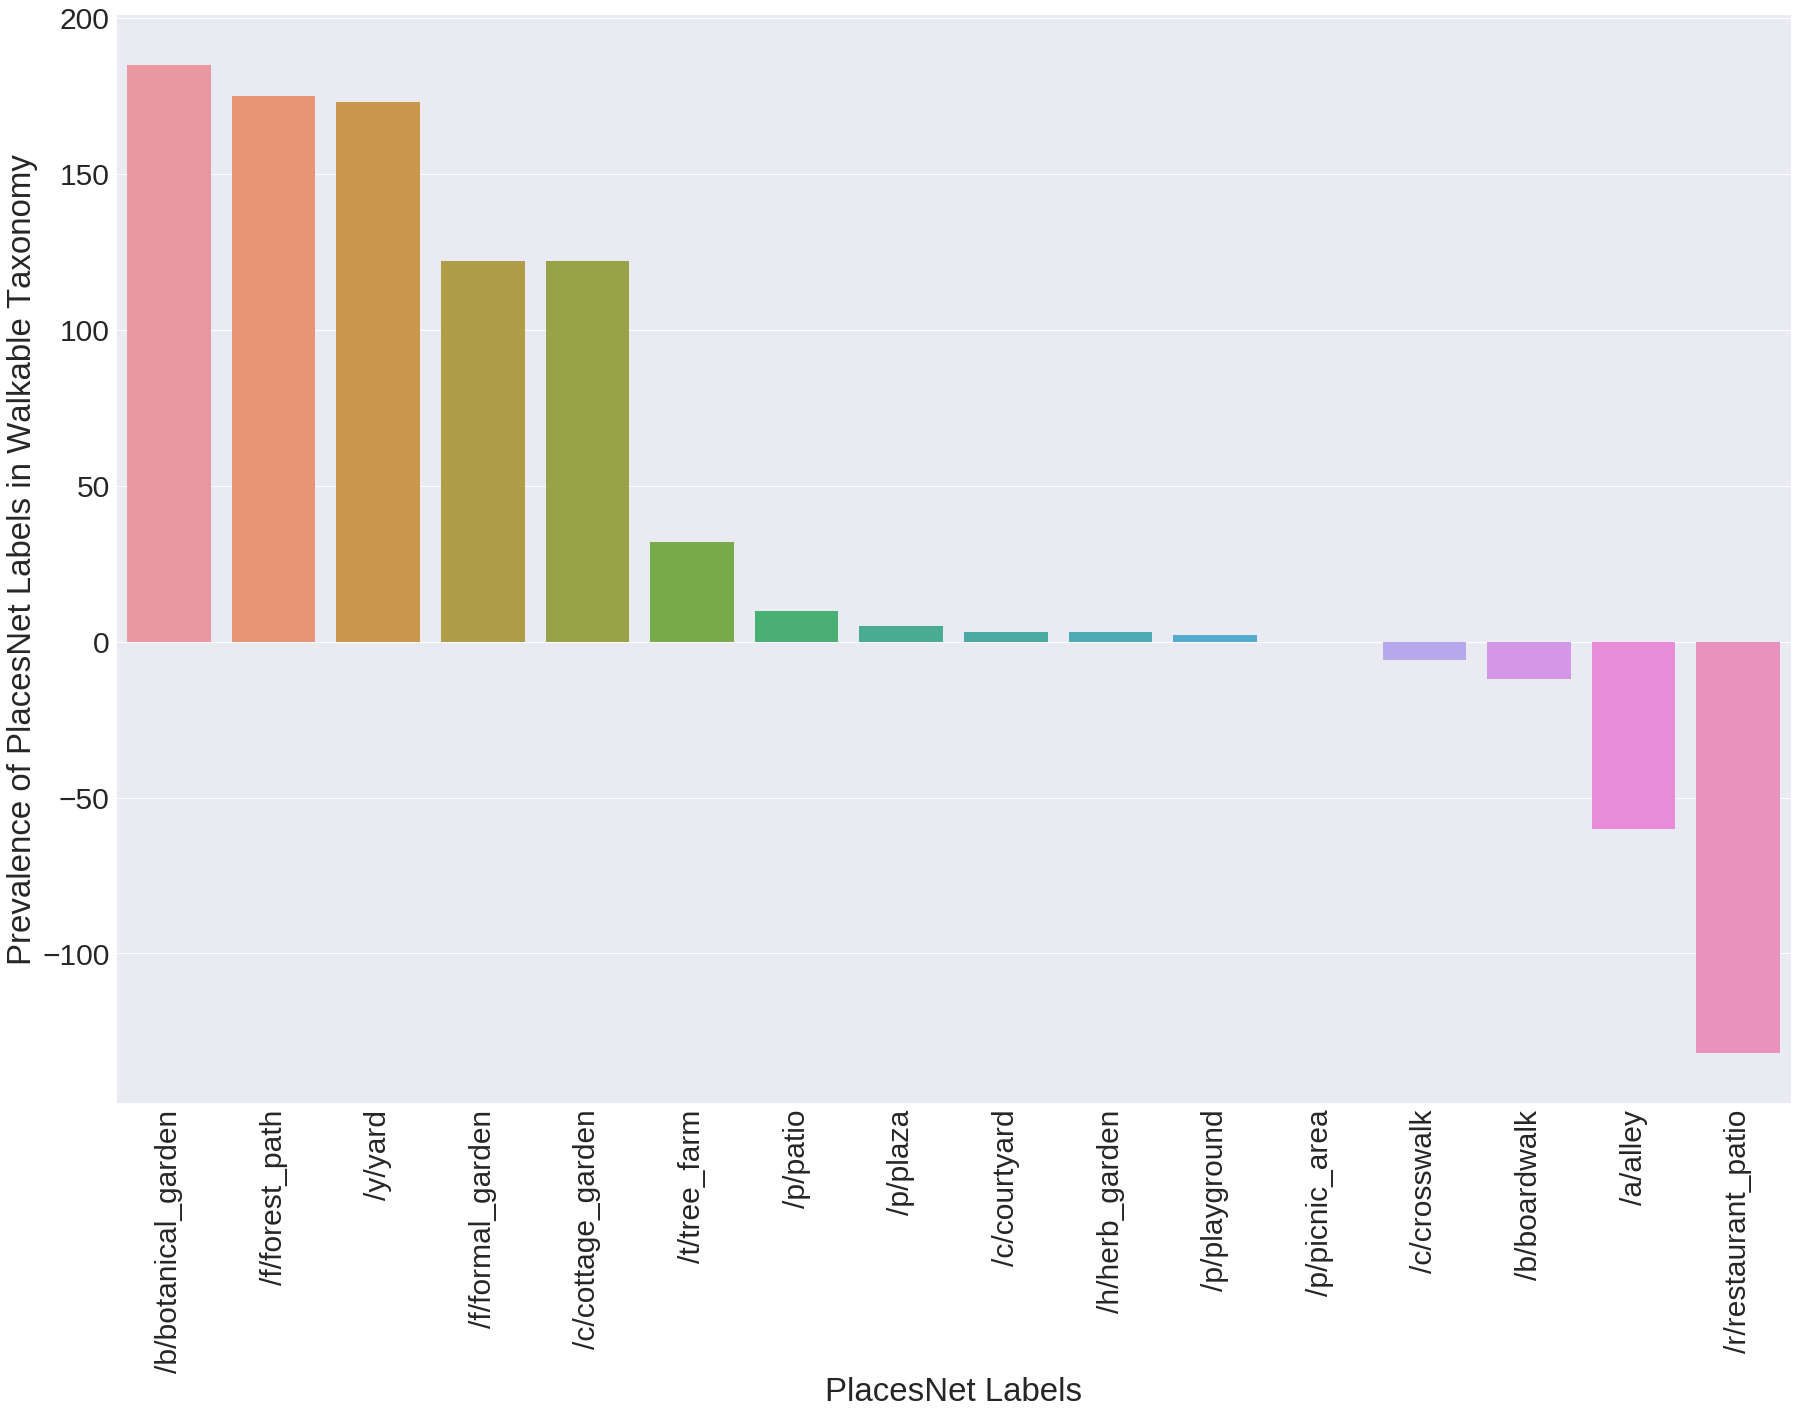
\includegraphics[width=\columnwidth]{Plot/walkable_taxonomy.png}
	\caption{Prevalence of Walkable labels in Beautified images against Ugly}
	\label{fig:WalkableTnomy}
\end{figure}

\begin{figure}[h]
	\centering
	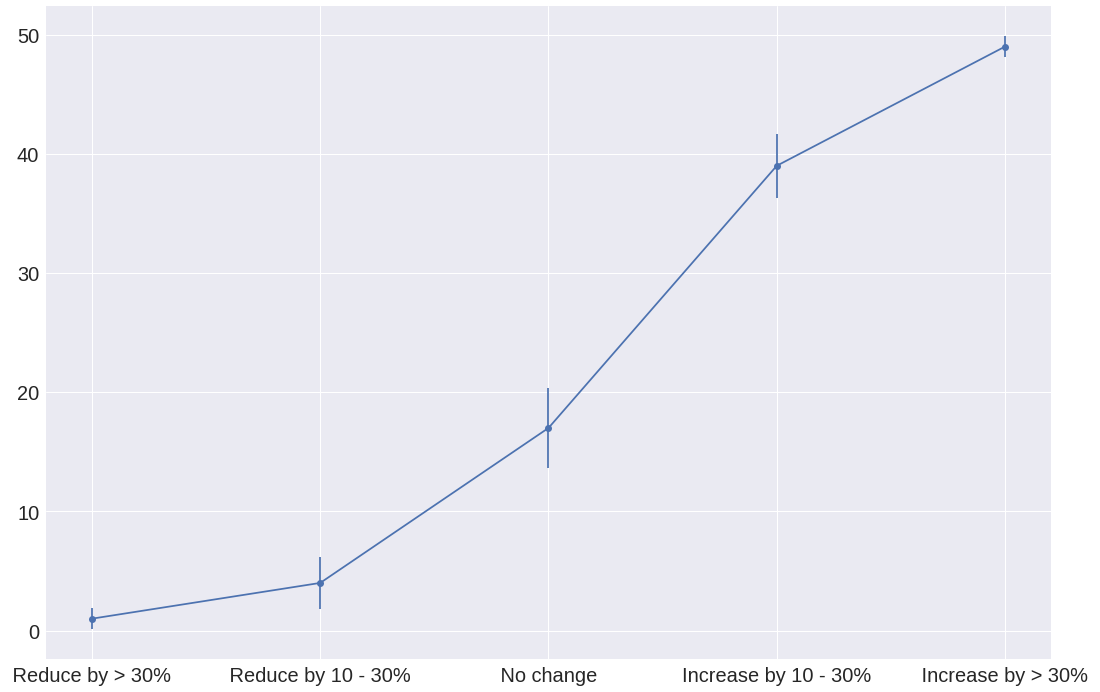
\includegraphics[width=\columnwidth]{Plot/Binned_deltas_trees.png}
	\caption{Binned Plot for greenery pixels across transfomed images}
	\label{fig:greenBinned}
\end{figure}


%\subsubsection{Vehicular traffic}
%\label{sec:vehicles}
%Vehicles are integral part of an urban scene. However when it comes to walk-ability of streets, higher traffic is not conducive. 
%This metric measures preference that the model puts on vehicular and road conditions. 
%\par
%\textit{[H3] Lesser vehicular traffic boosts walk-ability}
%\par
%The hypothesis states that for the same road dimensions, lesser vehicular traffic is preferential for beautiful urban scenes. 
%To test this we use Segnet \cite{badrinarayanan2015segnet}to extract pixels that belong to categories of road, cars, buildings etc. 
%In all Segnet supports 12 categories. The input to Segnet are the images transformed by our Top-Down pipeline on either side of the beauty spectrum. 
%We then calculate the change in proportion of road and car pixels. A positive change in road pixels suggests that the transformation added more road in the image. 
%From the distributions seen in Fig \ref{fig:roadCoverage} and Fig \ref{fig:vehicleCoverage}, there seems to be no significant change between original and transformed images in terms of road and vehicle pixels. This does not support \textbf{H3} , but 
%it does hint that the deep learning model did give a lot of preference on road and vehicle presence. 
%To understand the predictability and interdependence between presence of vehicles, presence of roads and the probability of finding an image beautiful, we adapt the approach as described in \cite{vaughn2008data}.
%Using the approach we perform a logistic regression over the two variables $V_i$ and $R_i$ which denote the ratio of area of vehicular pixels to the image area and the ratio of Road pixels to image area.
% Assuming dependence, we introduce another tern $VR_i$ which represents a composite of the two independent variables. 
%The logistic regression would try to fit a line 
%
%\begin{equation}
%	 L = \alpha + \beta_1 * V + \beta_2 * R  + \beta_3 * VR  
% \label{eq:regression} 
%\end{equation}
%
%
%In which case $L$ is a binary label for beautiful or ugly as transformed by the model, $V$ us a R.V for ratios for vehicle pixels across the dataset, $R$ is the R.V. for road pixels across the dataset and $VR$ is the product of two ratios. The regression yields $\alpha = 0$ , $\beta_1 = -0.003$ , $\beta_2 = -0.018$ and $\beta_3 = -0.68$. These values shed some light on dependence as well as individual influence of these variables , namely Roads and vehicles, on the beauty of an image as learned by the deep learning model. According to \cite{vaughn2008data}, the coefficients from equation \ref{eq:regression} approximate the influence of each variable on the outcome. 



\subsection{Privacy and  Openness }
From the literature, it is conjectured that privacy is great when one
looks at personal spaces, but when it comes to public settings, there is an inverse 'U' relation with how private a place feels like. 
Too much privacy, and it discourages the fundamental human urge to explore a mystery. Too much openness and it alerts the primal urge to feel safe. 
\par
\textit{[H3] Sense of Privacy has an inverse 'U' relationship with the sense of beauty }
\par
What \textit{H3} suggests is that sense of privacy is not always associated with beauty. 
To test this hypothesis we plot a binned plot of sky pixels across the dataset using the method described in Sec \ref{sec:Binned}. 

\begin{figure}[h]
	\centering
	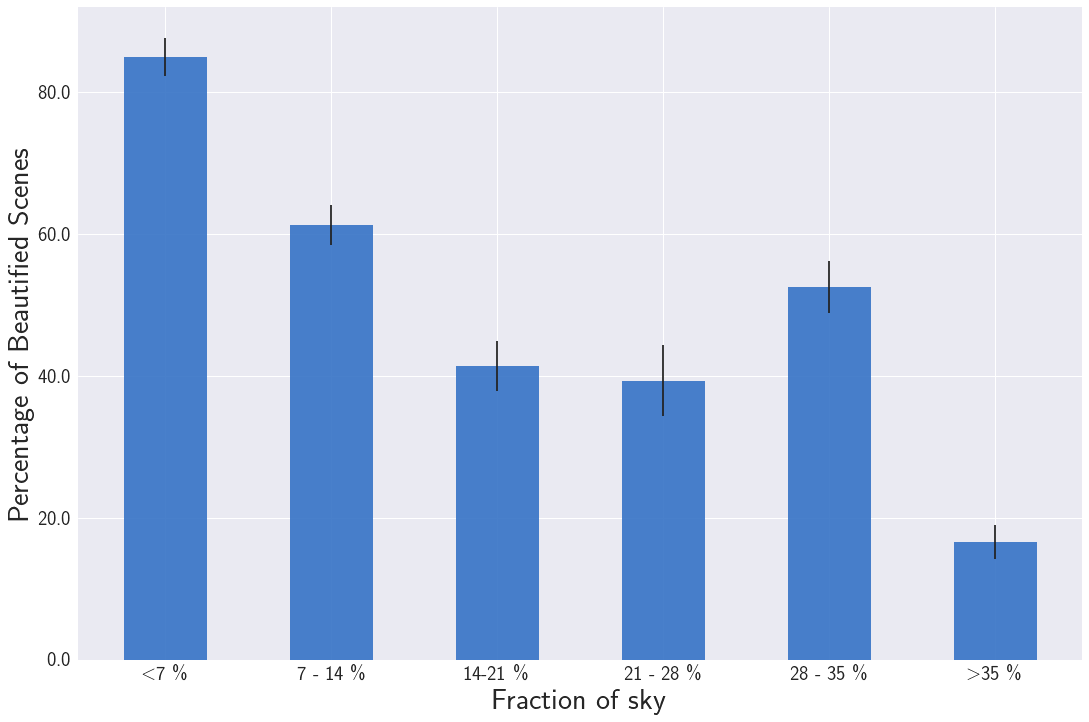
\includegraphics[width=\columnwidth]{Plot/BinnedPlot.png}
	\caption{Binned Plot for Sky pixels across transformed images}
	\label{fig:greenBinned}
\end{figure}

It can be seen that our model prefers lack of openness in the beautification process. The inverse 'U' Relationship is completely absent and cozy urban places are actually favoured in the beautification process. 

%This effect can be individually seen from Fig \ref{fig:BuildingsCoverage} and Fig \ref{fig:TreeCoverage}. Beautification always prefers reduction of 
%visible buildings and increase in an overall green coverage \footnote{All distributions are tested using student-t tests and are found to have significantly hight T-statistic score (>>20) and p value << $10^{-5}$}. However this does not necessarily untangle the trade-off relationship of privacy-openness and beauty.

%To understand relation between openness and privacy, we repeat analysis as described in Section \ref{sec:vehicles}, for the amount of Sky and Tree pixels in a scene. The assumption here is these two objects in the scene are predominately driving the sense of openness. Adapting the Equation \ref{eq:regression} for the tree and sky pixel ratios we get different values for $\beta_1 , \beta_2 and \beta_3$. In this case the regression yields $\alpha = 0$ , $\beta_1 = 0.06$ , $\beta_2 = 0.10$ and $\beta_3 = -0.04$ . These values suggest that trees and sky, on their own have a positive impact on the beauty of a picture. 

\subsection{Visual Complexity }
Visual complexity is a metric to measure the diversity of an urban scene. There is a trade off  when it comes to balancing visual complexity with beauty. Too much diversity overwhelms the cognition and makes it hard to establish bearing. To measure complexity, we treat the SegNet\cite{badrinarayanan2015segnet} labelled pixel proportions as a stochastic vector and find the Shannon Entropy on that vector for a given urban images. 
\begin{equation}
H(X) = -\sum p(i)\log p(i)
\label{eq:entropy} 
\end{equation}
The $i$ in Eq \ref{eq:entropy} is the segnet dimension for one of the 12 objects. This approximates complexity becasue the Segnet pixel proportions are stochastic in nature. It can be seen from Fig \ref{fig:complexity} that visual complexity does peak in beautiful images but then deteriorates rapidly.
\begin{figure}[h]
	\centering
	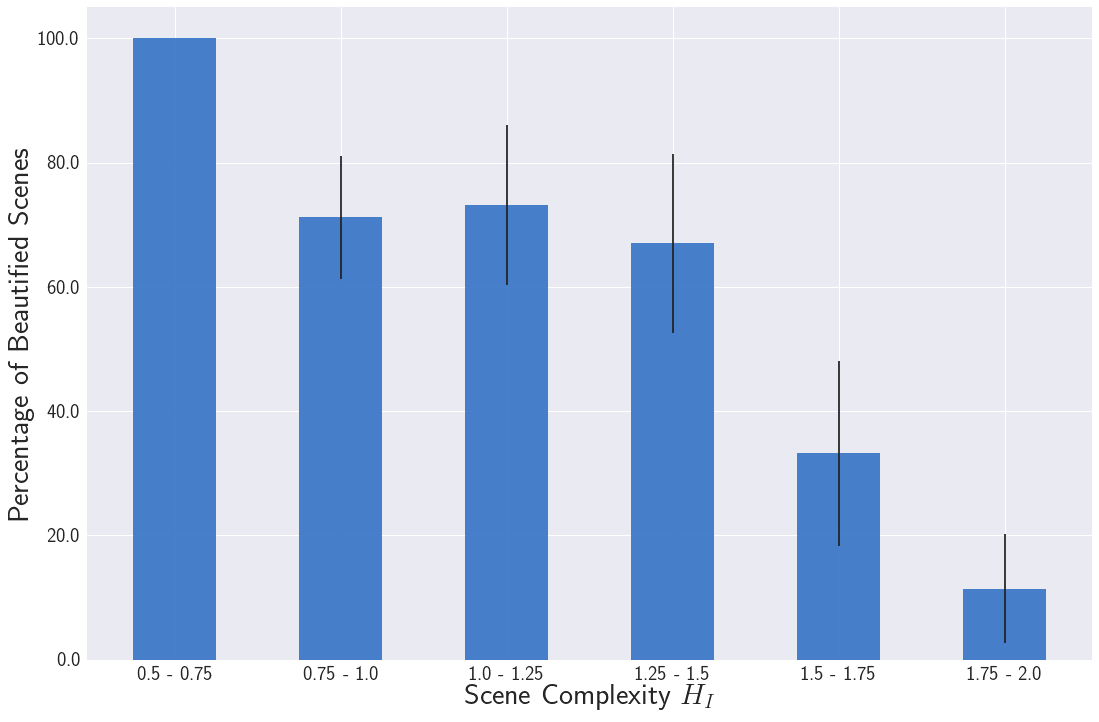
\includegraphics[width=\columnwidth]{Plot/binnedPlot_complexity.png}
	\caption{Binned Plot for Visual Complexity across transformed images}
	\label{fig:complexity}
\end{figure}







